% TODO famous example for a product line failure?

\subsection{Recap: Quality Assurance}
\begin{frame}{Recap: Software Quality} % caution: slide copied to analysis lecture
	\rightorleft{
		\mydefinition{Quality \mysource{\ludewiglichter}}{Quality is the entirety of properties and characteristics of a product or process that indicate adequacy with respect to given requirements.}
		\mydefinition{Quality Assurance \mysource{\ludewiglichter}}{Quality assurance \deutsch{Qualitätssicherung} are all activities with the goal to improve the quality.}
	}{
		\vspace{-12mm}
		\href{https://commons.wikimedia.org/wiki/File:Andy_Hunt_programmer.jpg}{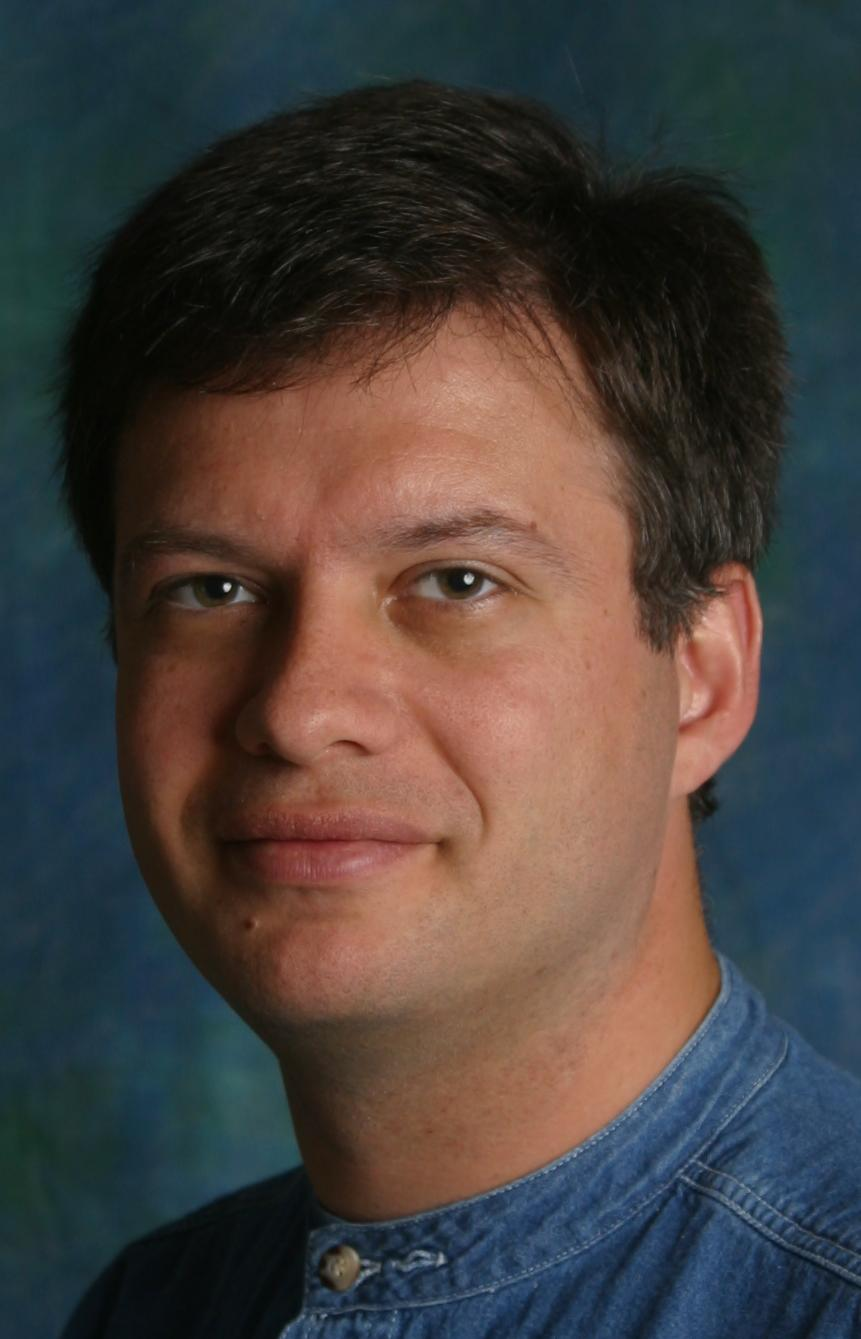
\includegraphics[width=\linewidth,trim=0 240 0 300,clip]{andy-hunt}}
		\vspace{-7mm}
		
		\mynote{Andy Hunt \mysource{\thepragmaticprogrammer}}{\mycite{No one in the brief history of computing has ever written a piece of perfect software. It's unlikely that you'll be the first.}}
		% co-authored The Pragmatic Programmer, known for the Agile Manifesto
	}
\end{frame}

\begin{frame}{Recap: Quality Assurance \mytitlesource{\ludewiglichter}} % caution: slide copied to analysis lecture
	\hfill%
	\only<1|handout:0>{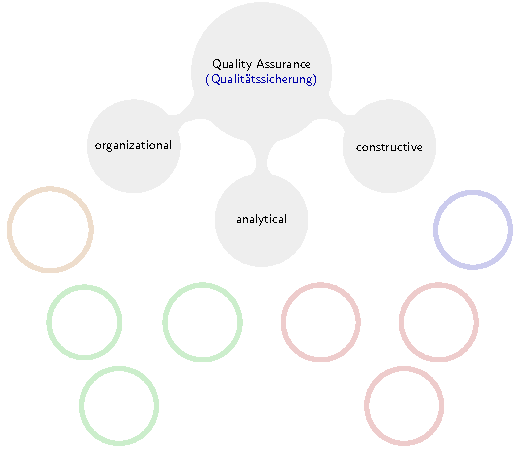
\includegraphics[height=\textheightwithtitle,page=1]{quality-assurance}}%
	\only<2|handout:0>{\includegraphics[height=\textheightwithtitle,page=2]{quality-assurance}}%
	\only<3|handout:0>{\includegraphics[height=\textheightwithtitle,page=3]{quality-assurance}}%
	\only<4|handout:0>{\includegraphics[height=\textheightwithtitle,page=4]{quality-assurance}}%
	\only<5|handout:1>{\includegraphics[height=\textheightwithtitle,page=5]{quality-assurance}}%
	\only<6|handout:0>{\includegraphics[height=\textheightwithtitle,page=7]{quality-assurance}}%
	% TODO check why this mindmap has a white background. could be large without a white background when using \textheightwithouttitle
\end{frame}

\begin{frame}{Recap: Software Testing}
	\leftorright{
		\vspace{7mm}
		\uncover<1-3>{\mydefinition{Software Testing \mysource{\sommerville}}{\mycite{Testing is intended to show that a program does what it is intended to do and to discover program defects before it is put into use.}}{}}
		\uncover<2-3>{\mydefinition{Validation Testing \mysource{\sommerville}}{\mycite{Demonstrate to the developer and the customer that the software meets its requirements.}}{}}
		\uncover<3-3>{\mydefinition{Defect Testing \mysource{\sommerville}}{\mycite{Find inputs or input sequences where the behavior of the software is incorrect, undesirable, or does not conform to its specification.}}{}}
	}{
		\vspace{-12mm}
		\uncover<4>{\mynote{V\&V \mysource{\seeconomics}}{\mycite{\emph{Validation}: Are we building the right product?\\\emph{Verification}: Are we building the product right?}}} 
		% TODO better visualization of V&V (see Inas slides). move to V model?
		\vspace{-2mm}
		\uncover<5>{\mynote{Stages of Testing \mysource{\sommerville}}{
			\begin{itemize}
				\setlength\itemsep{.1em}
				\item[1.] \mycite{\emph{Development testing}, where the system is tested during development to discover
				bugs and defects}
				\item[2.] \mycite{\emph{Release testing}, where a separate testing team tests a complete version of the
				system before it is released to users}
				\item[3.] \mycite{\emph{User testing}, where users or potential users of a system test the system in their
				own environment}
			\end{itemize}
		}}
		\vspace{-2mm}
		\uncover<6>{\mynote{}{\mycite{In \emph{manual testing}, a tester runs the program with some test data and
				compares the results to their expectations. [...] In \emph{automated testing}, the tests are encoded in a program that is run each time the system under development is to be tested.} \mysource{\sommerville}}}
	}
\end{frame}

\begin{frame}
	\leftorright{
		\href{https://commons.wikimedia.org/wiki/File:Edsger_Wybe_Dijkstra.jpg}{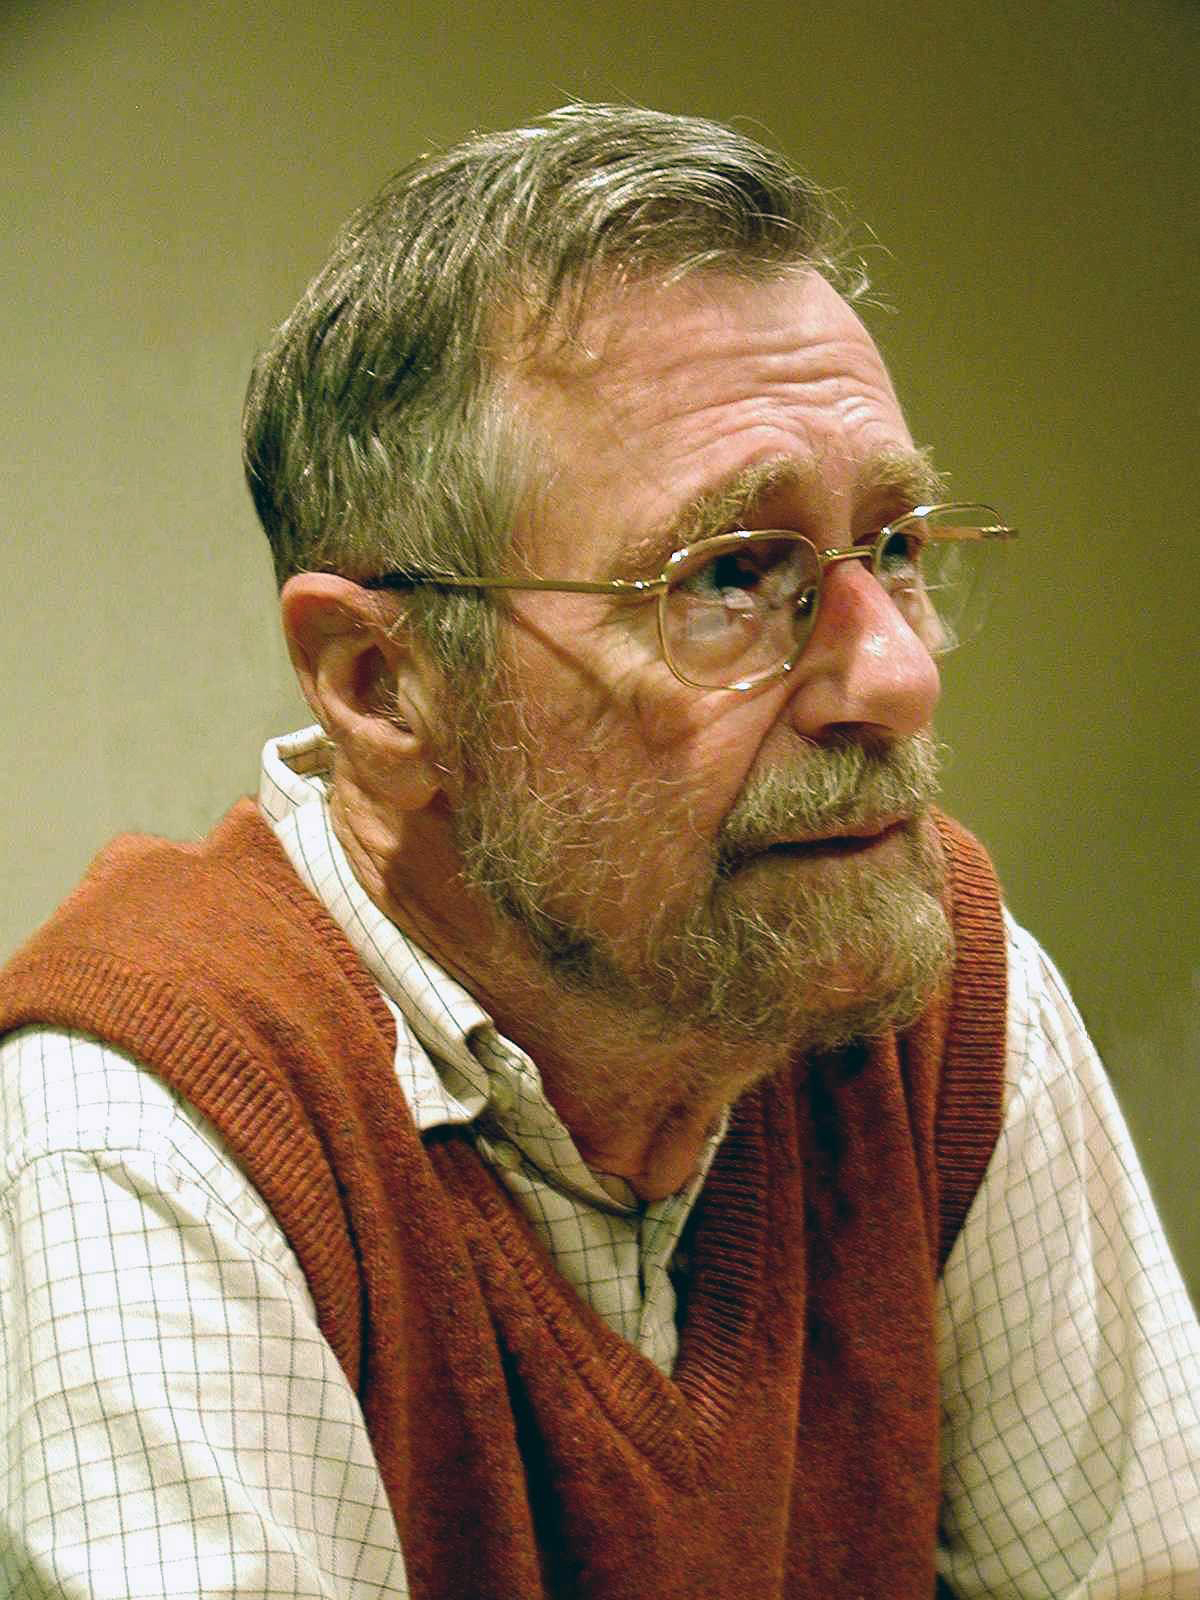
\includegraphics[width=\linewidth,trim=0 425 0 75,clip]{edsger-dijkstra}}
		\vspace{-7mm}
		
		\mynote{Edsger W. Dijkstra (1972) \mysource{\thehumbleprogrammer}}{\mycite{Program testing can be a very effective way to show the presence of bugs, but it is hopelessly inadequate for showing their absence.}}
		% 1930-2002, ACM Turing Award winner
	}{
		\todo{illustration for many configurations from previous slides}
	}
\end{frame}

\subsection{Testing All Configurations}
\begin{frame}{\insertsubsection}
	\leftorright{
		\centering\featureDiagramConfigurableDatabase
		
		\myexample{Recap: 26 Valid Configurations \lecturemodeling}{
			\todo{update list based on the example (here and on later slides)}

			\footnotesize
			\leftandright{
				$\{B,G,W\}$\\
				$\{B,P,W\}$\\
				$\{B,G,P,W\}$\\
				$\{B,D,W\}$\\
				$\{B,G,D,W\}$\\
				$\{B,P,D,W\}$\\
				$\{B,G,P,D,W\}$\\
				$\{B,P,T,W\}$\\
				$\{B,G,P,T,W\}$\\
				$\{B,D,T,W\}$\\
				$\{B,G,D,T,W\}$\\
				$\{B,P,D,T,W\}$\\
				$\{B,G,P,D,T,W\}$
			}{
				$\{B,G,U\}$\\
				$\{B,P,U\}$\\
				$\{B,G,P,U\}$\\
				$\{B,D,U\}$\\
				$\{B,G,D,U\}$\\
				$\{B,P,D,U\}$\\
				$\{B,G,P,D,U\}$\\
				$\{B,P,T,U\}$\\
				$\{B,G,P,T,U\}$\\
				$\{B,D,T,U\}$\\
				$\{B,G,D,T,U\}$\\
				$\{B,P,D,T,U\}$\\
				$\{B,G,P,D,T,U\}$
			}
		}
	}{
		\vspace{-7mm}
		\mynote{Discussion}{
			\begin{itemize}
				\setlength\itemsep{.5em}
				\item only feasible for small product lines (few valid configurations)
				\item redundant test effort
				\item large product lines: not even feasible to generate and compile all configurations
				\item (some) large product lines: not even the number of valid configurations is known
			\end{itemize}
		}
		\myexampletight{\small Recap: Industrial Configuration Spaces \lecturemodeling}{
			\centering\evaluatingsharpsatsolverslink{\includegraphics[width=.8\linewidth,page=6,trim=50 210 320 440,clip]{2020/2020-VaMoS-Sundermann}}
		}
	}
\end{frame}

\begin{frame}{Recap: Feature Model of the Linux Kernel}
	\vspace{28mm}~\hspace{-15mm}\href{https://dl.acm.org/doi/abs/10.1145/3382025.3414943}{\includegraphics[width=1.2\linewidth,page=1,trim=100 510 100 170,clip]{2020/2020-SPLC-Thuem}}
\end{frame}

\newcommand{\eemph}[1]{{\color{red}\textbf{#1}}}

\subsection{Testing One Configuration}
\begin{frame}{\insertsubsection}
	\leftorright{
		\centering\featureDiagramConfigurableDatabase
		
		\myexample{Which Valid Configuration to Test?}{
			\footnotesize
			\leftandright{
				$\{B,G,W\}$\\
				$\{B,P,W\}$\\
				$\{B,G,P,W\}$\\
				$\{B,D,W\}$\\
				$\{B,G,D,W\}$\\
				$\{B,P,D,W\}$\\
				$\{B,G,P,D,W\}$\\
				$\{B,P,T,W\}$\\
				$\{B,G,P,T,W\}$\\
				$\{B,D,T,W\}$\\
				$\{B,G,D,T,W\}$\\
				$\{B,P,D,T,W\}$\\
				\eemph{$\{B,G,P,D,T,W\}$}
			}{
				$\{B,G,U\}$\\
				$\{B,P,U\}$\\
				$\{B,G,P,U\}$\\
				$\{B,D,U\}$\\
				$\{B,G,D,U\}$\\
				$\{B,P,D,U\}$\\
				$\{B,G,P,D,U\}$\\
				$\{B,P,T,U\}$\\
				$\{B,G,P,T,U\}$\\
				$\{B,D,T,U\}$\\
				$\{B,G,D,T,U\}$\\
				$\{B,P,D,T,U\}$\\
				\emph{$\{B,G,P,D,T,U\}$}
			}
		}
	}{
		\mynote{Discussion}{
			\begin{itemize}
				\setlength\itemsep{.4em}
				\item applicable to large product lines
				\item no redundant test effort (from configurations)
				\item often not feasible to test all features in one configuration (e.g., Win and Unix)
				\item strategy in practice: all-yes-config (configuration with many features selected)
				\item unnoticed feature interactions \lectureinteractions
			\end{itemize}
		}
		\todo{picture on known interaction from \lectureinteractions}
	}
\end{frame}

% Dijkstra: we cannot test everything, and not all configurations
% complete test: all inputs, for all products/variants/configurations
% sampling technique (Stichprobenverfahren)
% recap: Testing All Configurations (remember numbers from intro? take 1ms per config)
% recap: Testing One Configuration (cp. allyesconfig, feature interactions may not be visible)

\subsection{Expert Knowledge in Sampling}

\subsection{Random Sampling}

\subsection{Excursus: Uniform Random Sampling}

\subsection{Testing the Linux Kernel}
% allyesconfig

%\subsection{Automation in Product Sampling} ???

%\subsection{Missing: Test-Case Selection/Generation}
% What to test for those configurations? Variable unit tests? Avoid redundant testing?

% TODO how Linux is developed: patches on mailing list, only considered if not rejected by CI, what happens in CI

